\documentclass[12pt]{article}

\usepackage{amsfonts, amsmath, amssymb, amstext, latexsym}
\usepackage{graphicx, epsfig}
\usepackage[utf8]{inputenc}
\usepackage[french]{babel}
\usepackage{exscale}
\usepackage{amsbsy}
\usepackage{amsopn}
\usepackage{fancyhdr}

\usepackage{amsmath, amssymb, amsfonts, amsthm, fouriernc, mathtools}
% mathtools for: Aboxed (put box on last equation in align envirenment)
\usepackage{microtype} %improves the spacing between words and letters

\usepackage{graphicx}
\usepackage{epsfig}
\usepackage{epstopdf}

%%%%%%%%%%%%%%%%%%%%%%%%%%%%%%%%%%%%%%%%%%%%%%%%%%
%% COLOR DEFINITIONS
%%%%%%%%%%%%%%%%%%%%%%%%%%%%%%%%%%%%%%%%%%%%%%%%%%
\usepackage[svgnames]{xcolor} % Enabling mixing colors and color's call by 'svgnames'
%%%%%%%%%%%%%%%%%%%%%%%%%%%%%%%%%%%%%%%%%%%%%%%%%%
\definecolor{MyColor1}{rgb}{0.2,0.4,0.6} %mix personal color
\newcommand{\textb}{\color{Black} \usefont{OT1}{lmss}{m}{n}}
\newcommand{\blue}{\color{MyColor1} \usefont{OT1}{lmss}{m}{n}}
\newcommand{\blueb}{\color{MyColor1} \usefont{OT1}{lmss}{b}{n}}
\newcommand{\red}{\color{LightCoral} \usefont{OT1}{lmss}{m}{n}}
\newcommand{\green}{\color{Turquoise} \usefont{OT1}{lmss}{m}{n}}
%%%%%%%%%%%%%%%%%%%%%%%%%%%%%%%%%%%%%%%%%%%%%%%%%%


\usepackage{fullpage}
\usepackage{amsmath}
\usepackage{graphicx}
\usepackage{caption}
\usepackage{amsthm}
\usepackage{float}
\usepackage{amssymb}

%%%%%%%%%%%%%%%%%%%%%%%%%%%%%%%%%%%%%%%%%%%%%%%%%%
%% FONTS AND COLORS
%%%%%%%%%%%%%%%%%%%%%%%%%%%%%%%%%%%%%%%%%%%%%%%%%%
%    SECTIONS
%%%%%%%%%%%%%%%%%%%%%%%%%%%%%%%%%%%%%%%%%%%%%%%%%%
\usepackage{titlesec}
\usepackage{sectsty}
%%%%%%%%%%%%%%%%%%%%%%%%
%set section/subsections HEADINGS font and color
\sectionfont{\color{MyColor1}}  % sets colour of sections
\subsectionfont{\color{MyColor1}}  % sets colour of sections

%set section enumerator to arabic number (see footnotes markings alternatives)
\renewcommand\thesection{\arabic{section}.} %define sections numbering
\renewcommand\thesubsection{\thesection\arabic{subsection}} %subsec.num.

%define new section style
\newcommand{\mysection}{
\titleformat{\section} [runin] {\usefont{OT1}{lmss}{b}{n}\color{MyColor1}}
{\thesection} {3pt} {} }

%%%%%%%%%%%%%%%%%%%%%%%%%%%%%%%%%%%%%%%%%%%%%%%%%%
%		CAPTIONS
%%%%%%%%%%%%%%%%%%%%%%%%%%%%%%%%%%%%%%%%%%%%%%%%%%
\usepackage{caption}
\usepackage{subcaption}
%%%%%%%%%%%%%%%%%%%%%%%%
\captionsetup[figure]{labelfont={color=Turquoise}}

%%%%%%%%%%%%%%%%%%%%%%%%%%%%%%%%%%%%%%%%%%%%%%%%%%
%		!!!EQUATION (ARRAY) --> USING ALIGN INSTEAD
%%%%%%%%%%%%%%%%%%%%%%%%%%%%%%%%%%%%%%%%%%%%%%%%%%
%using amsmath package to redefine eq. numeration (1.1, 1.2, ...)
%%%%%%%%%%%%%%%%%%%%%%%%
\renewcommand{\theequation}{\thesection\arabic{equation}}

%set box background to grey in align environment
\usepackage{etoolbox}% http://ctan.org/pkg/etoolbox
\makeatletter
\patchcmd{\@Aboxed}{\boxed{#1#2}}{\colorbox{black!15}{$#1#2$}}{}{}%
\patchcmd{\@boxed}{\boxed{#1#2}}{\colorbox{black!15}{$#1#2$}}{}{}%
\makeatother
%%%%%%%%%%%%%%%%%%%%%%%%%%%%%%%%%%%%%%%%%%%%%%%%%%




%%%%%%%%%%%%%%%%%%%%%%%%%%%%%%%%%%%%%%%%%%%%%%%%%%
%% DESIGN CIRCUITS
%%%%%%%%%%%%%%%%%%%%%%%%%%%%%%%%%%%%%%%%%%%%%%%%%%
\usepackage[siunitx, american, smartlabels, cute inductors, europeanvoltages]{circuitikz}
%%%%%%%%%%%%%%%%%%%%%%%%%%%%%%%%%%%%%%%%%%%%%%%%%%



\makeatletter
\let\reftagform@=\tagform@
\def\tagform@#1{\maketag@@@{(\ignorespaces\textcolor{red}{#1}\unskip\@@italiccorr)}}
\renewcommand{\eqref}[1]{\textup{\reftagform@{\ref{#1}}}}
\makeatother
\usepackage{hyperref}
\hypersetup{colorlinks=true}

%%%%%%%%%%%%%%%%%%%%%%%%%%%%%%%%%%%%%%%%%%%%%%%%%%
%% PREPARE TITLE
%%%%%%%%%%%%%%%%%%%%%%%%%%%%%%%%%%%%%%%%%%%%%%%%%%
\title{\blue Principes et Méthodes Statistiques \\
\blueb TP 2017}
\author{Pierre Bouvier, Nolwenn Cadic, Maxime Gourgoulhon}
\date{\today}
%%%%%%%%%%%%%%%%%%%%%%%%%%%%%%%%%%%%%%%%%%%%%%%%%%

\newcommand{\noi}{\noindent}
\newcommand{\dsp}{\displaystyle}

\textheight 25cm
\textwidth 16cm
\oddsidemargin 0cm
\evensidemargin 0cm
\topmargin 0cm
\hoffset -0mm
\voffset -20mm


\pagestyle{plain}


\begin{document}

\maketitle
\baselineskip7mm

% \noi ENSIMAG $1^{\footnotesize \mbox{ère}}$ année   \hfill Mars 2017


\vspace{1cm}


\begin{center}
{\Large \bf Principes et Méthodes Statistiques

\vspace{3mm}

TP 2017

\vspace{3mm}

}
\end{center}

\noi \rule[0.5ex]{\textwidth}{0.1mm}


\section*{Introduction au problème}

Les données considérées sont issues d'une démarche d'analyse de signaux oculométri-ques, c'est-à-dire de signaux de suivi du mouvement des yeux au cours du temps. Ces signaux ont été mesurés sur des participants lors de tâches consistant à lire des textes traitant de thèmes prédéfinis : football, chasse aux oiseaux, physique nucléaire, art contemporain, etc...
L'objectif est que le lecteur identifie le thème du texte le plus vite possible.

Lors de la lecture, deux types de mouvements d'yeux alternent : la fixation, qui correspond à la lecture proprement dite d'un mot ou deux voire moins, et où les yeux sont quasi-immobiles, et la saccade, qui est un déplacement très rapide portant les yeux vers un autre mot ou une autre partie d'un mot long.

On considère un premier groupe de $n=227$ personnes à qui on a fait lire $n$ textes pris au hasard dans une première série de textes. On mesure pour chaque personne le nombre $X$ de fixations nécessaires pour identifier le type du texte lu. Les données sont fournies dans le fichier {\it groupe1.txt}.
Le fichier {\it groupe2.txt} contient des données similaires pour un second groupe de $m=168$ personnes à qui on a fait lire $m$ textes pris au hasard dans une autre série de textes.

L'objectif du TP est d'analyser ces données et de comparer les 2 groupes. On propose de modéliser la loi de probabilité de $X$ par une loi géométrique ou une loi binomiale négative.


%%%%%%%%%%%%%%%%%%%%%%%%%%%%%%%%%%%%%%%%%%%%%%%%%%%%%%%%%%%%%%%
\section{Analyse d'échantillons de loi binomiale négative}
%%%%%%%%%%%%%%%%%%%%%%%%%%%%%%%%%%%%%%%%%%%%%%%%%%%%%%%%%%%%%%%

Une variable aléatoire $X$ est de loi binomiale négative ${\cal BN}(r,p)$ de paramètres $r \in \mathbb{N}^*$ et $p \in [0, 1]$  si elle est à valeurs dans $ \{r, r+1, ...\}$ et que :
$$P(X=x) = \binom{x-1}{r-1}(1-p)^{x-r}p^r, \, \forall x \in \{r, r+1, ...\}$$

Son espérance est $E[X]={\dsp \frac{r}{p}}$ et sa variance est $Var[X]={\dsp \frac{r(1-p)}{p^2}}$.

En {\tt R}, {\tt rnbinom(n,r,p)} simule un échantillon de taille $n$ d'une variable aléatoire $Y$ telle que $Y+r$ est de loi ${\cal BN}(r,p)$.

La loi géométrique ${\cal G}(p)$ est la loi ${\cal BN}(1,p)$. En {\tt R}, {\tt rgeom(n,p)} simule un échantillon de taille $n$ d'une variable aléatoire $Y$ telle que $Y+1$ est de loi ${\cal G}(p)$.

On considère un échantillon $X_1, \ldots, X_n$ de variables aléatoires indépendantes et de même loi ${\cal BN}(r,p)$.

Dans un premier temps, on suppose que le paramètre $r$ est connu.

\vspace{3mm}

\begin{enumerate}

\renewcommand{\labelenumi}{\arabic{section}.\arabic{enumi}.}

\item Estimer $p$ par la méthode des moments, puis par la méthode de maximum de vraisemblance. Montrer que les deux estimateurs sont égaux. On notera $\hat{p}_n$ cet estimateur.

\textbf{Réponse :\\}
\underline{méthode des moments :} $E[X] = \dsp \frac{r}{p} \Rightarrow p = \frac{e}{E[X]} \Rightarrow \hat{p}_n = \frac{r}{\bar{X}_n} $ \\
\underline{méthode du maximum de vraisemblance :} \\
Soit  la fonction de vraisemblance $\mathcal{L}(p, r, x_{1}, ..., x_{n})$,\\$$\mathcal{L}(p, r, x_{1}, ... , x_{n}) = \prod_{i=1}^{n}P(X=x_{i}, p, r)  = \prod_{i=1}^n \binom{x_i-1}{r-1}(1-p)^{x_i-r}p^r$$ \\
On cherche à trouver le minimum de cette fonction par rapport à p. \\
\[\frac{\partial{ln(\mathcal{L}(p, r, x_{1}, ... , x_{n}))}}{\partial{p}} = -\sum_{i=1}^{n} \frac{x_{i}}{1-p} + \frac{rn}{p(1-p)}\]
\[\frac{\partial{ln(\mathcal{L}(p, r, x_{1}, ... , x_{n}))}}{\partial{p}} = 0 \Rightarrow \frac{rn}{p} = -\sum_{i=1}{n} x_{i} \Rightarrow \hat{p}_n = \frac{r}{\bar{X}_n}\]
\vspace{3mm}

\item Appliquer le théorème central-limite à $\bar{X}_n$. En déduire un intervalle de confiance bilatéral asymptotique de seuil $\alpha$ pour $p$.

$$ IC = \left[ \frac{r}{\bar{X}_n} - u_{\alpha} \sqrt{r\frac{\bar{X}_n - r}{n\bar{X}_n^3}} ,\,\, \frac{r}{\bar{X}_n} + u_{\alpha} \sqrt{r\frac{\bar{X}_n - r}{n\bar{X}_n^3}}  \right] $$

\vspace{3mm}

\item Dans le cas de la loi géométrique ($r=1$), construire le graphe de probabilités avec la méthode usuelle basée sur la fonction de répartition. En déduire une estimation graphique $p_{g_1}$ de $p$. Evaluer la qualité de cette méthode sur la base de jeux de données simulées.

\textbf{Réponse : \\}
Calcul de la fonction de répartition pour le graphe : $$ F(k) = P(X \leq k) = \sum_{i=1}^{k} q^{i-1}p = p\sum_{i=0}^{n-1} q^{i} = 1 - q^{k}$$
On a $$ 1 - F(k) = q_{k} \Rightarrow ln(1-F(k)) = k ln(q)$$
On pose $H(x) = ln(1-x)$ et $g(x) = x$ et on obtient comme graphe de probabilité pour la fonction de répartition le nuage de points $ (g(x_i^{*}), \; h(\frac{i}{n})) \quad \forall i \in \llbracket 1; n \rrbracket $
\begin{center}
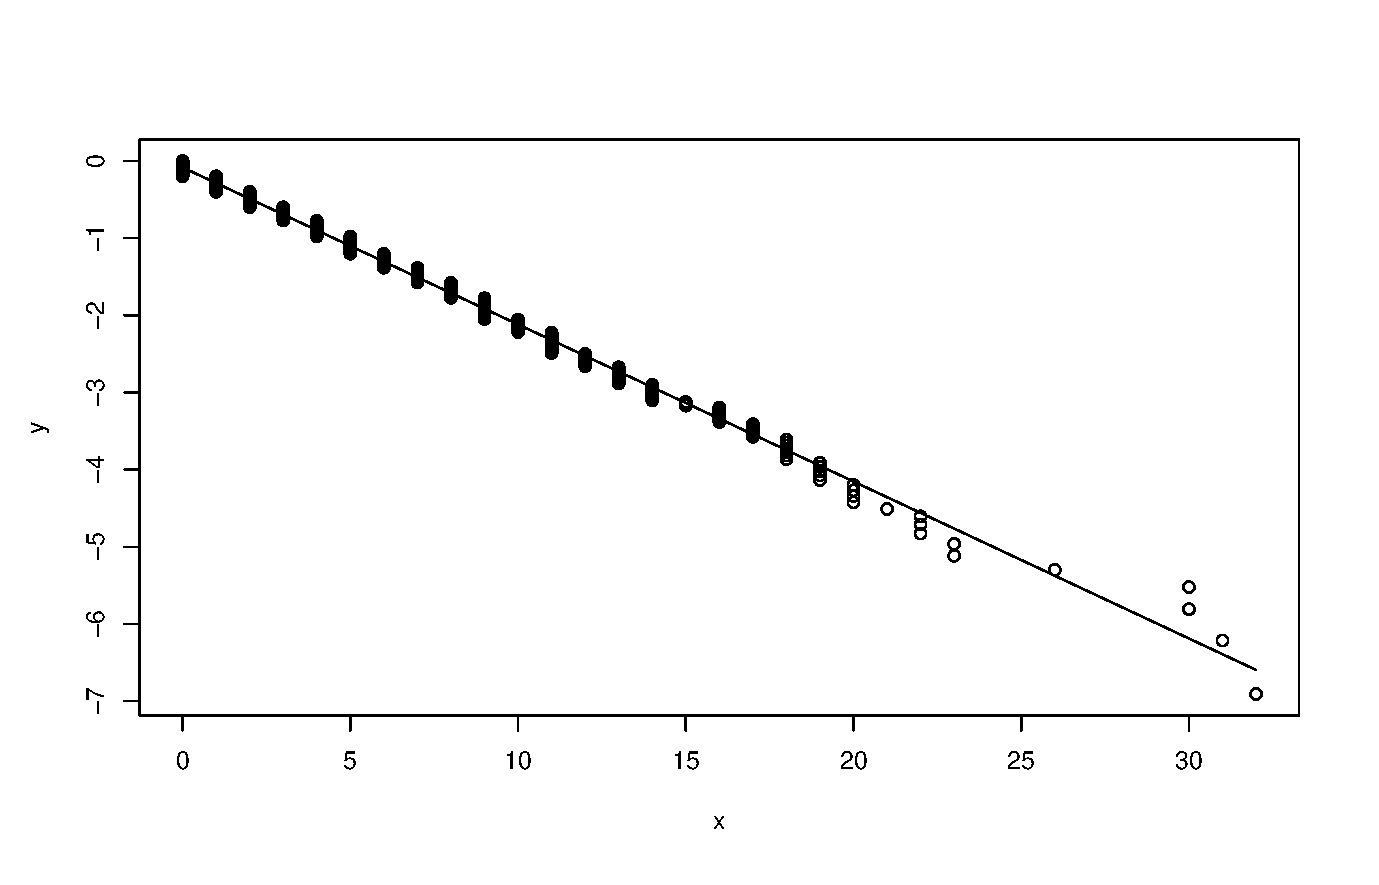
\includegraphics[width=15cm]{{{graphics/q1.3}.eps}}
\label{fig1}
\end{center}
Pour réaliser ce graphe, nous avons simulés avec $n = 1000$ et $p = 0.1789$. \\
Après une régression affine, nous avons comme pente: $-0.1965$. \\
Ainsi on estime graphiquement $p_{g_1} = e^{-0.1965} = 0.1784196$.
Après tests avec d'autres paramètres, nous trouvons aussi de très bons résultats: l'estimateur est d'excellente qualité. \\
\vspace{3mm}

\item Dans le cas de la loi binomiale négative avec $r>1$, cette méthode ne fonctionne pas car la fonction de répartition n'a pas d'expression simple. On propose alors une méthode similaire basée sur un autre critère.

\begin{enumerate}

\vspace{3mm}

\item Quand $X$ est de loi ${\cal BN}(r,p)$, calculer ${\dsp \frac{P(X=x)}{P(X=x+1)}}$.

\textbf{Réponse :\\}
$$\frac{P(X=x)}{P(X=x+1)} = \frac{\binom{x-1}{r-1} (1-p)^{x-r} p^{r}}{\binom{x}{r-1} (1-p)^{x-r+1} p^{r}} = \frac{1}{1-p} \frac{x-r+1}{x}$$

\vspace{3mm}

\item Proposer une méthode permettant d'évaluer à partir d'un nuage de points si la loi Binomiale Négative est un modèle plausible. En déduire deux estimations graphiques de $p$, $p_{g_2}$ et $p_{g_3}$.

\textbf{Réponse :\\}
Comme nous avons l'égalité suivante: $x \dsp \frac{P(X=x)}{P(X=x+1)} = \frac{x}{1-p} +\frac{r-1}{p-1}$ \\
Nous traçons les points suivants: $\left({x_i^\#} ; x_i^\# \dsp \frac{P(X=x_i^\#)}{P(X=x_{i}^\# + 1)} \right)$ \\
Où $x_i^\#$ vaut 0 quand $i$ n'a pas été tiré sinon $i$
Nous calculons sa droite de régression affine, notons son résultat: Y=Ax+B. \\
On pose: $A = \frac{1}{1-p_{g_2}}$ et $B = \frac{r-1}{p_{g_3}-1}$. \\
Ainsi: $p_{g_2} = 1 - \frac{1}{A}$ et $p_{g_3} = 1 + \frac{r-1}{B}$
\vspace{3mm}

\item Evaluer la qualité de cette méthode sur la base de jeux de données simulées.

\end{enumerate}

\vspace{3mm}

En simulant un grand nombre de fois avec des paramètres n, r, p différents, on peut en déduire que les estimateurs sont peu précis pour p faible, et que plus p est grand, plus ils deviennent précis. \\
Les estimateurs donnent soit des résultats abhérents, soit des estimations biaisées: il est facile à mettre en évidence dans notre code, les p estimés quasi-systématiquement surestimés, et quand on on augmente, ce biais augmente. \\

\hspace{-5mm} Dans un deuxième temps, on considère que les 2 paramètres $p$ et $r$ sont inconnus.

\vspace{3mm}

\item Calculer les estimateurs de $p$ et $r$ par la méthode des moments, $\tilde{p}_n$ et $\tilde{r}_n$.

\textbf{Réponse:\\}
On a, $ \dsp \frac{Var[X]}{E[X]} = \frac{1-p}{n} = \frac{1}{p} - 1 \Rightarrow \tilde{p}_n = \frac{\bar{X}_n}{S_n+\bar{X}_n} $ \\
Puisque $ r= p E[X]$, on obtient $\dsp \tilde{r}_n = \frac{ \bar{X}_n^2}{S_n + \bar{X}_n} $
\vspace{3mm}

\item Proposer une méthode numérique permettant de calculer les estimateurs de maximum de vraisemblance $\hat{p}_n$ et $\hat{r}_n$.

\textbf{Réponse :\\}
On peut aisément calculer p, si l'on connait r.
Par définition, $X$ est à valeurs dans \{$r, r+1, ..., +\infty$\}, on sait donc que $r \leq min(x_i)$.
Il suffit alors d'énumérer les r possibles pour pouvoir trouver le couple (r, p) maximisant la vraisemblance. \\
Voici notre algorithme:
\begin{verbatim}
Fonction estimer_p_et_r(données):
    vraisemblance = $-\infty$
    meilleur_r = -1
    p_associe = -1
    Pour $r_i$ entier appartenant à $[1, min(données)]$:
        nouveau_p = calcul_maximum_vraisemblance_pour_p($r_i$, données)
        nouvelle_vraisemblance = calcul_vraisemblance(nouveau_p, $r_i$, données)
        Si nouvelle_vraisemblance > vraisemblance:
            meilleur_r = $r_i$
            p_associe = nouveau_p
            vraisemblance = nouvelle_vraisemblance
        Fin Si
    Fin pour
Retourner meilleur_r et p_associé
\end{verbatim}
\end{enumerate}


%%%%%%%%%%%%%%%%%%%%%%%%%%%%%%%%%%%%%%%%%%%%%%%%%%%%%%%%%%%%%%%
\section{Analyse des deux jeux de données}
%%%%%%%%%%%%%%%%%%%%%%%%%%%%%%%%%%%%%%%%%%%%%%%%%%%%%%%%%%%%%%%

\begin{enumerate}

\renewcommand{\labelenumi}{\arabic{section}.\arabic{enumi}.}

\item Effectuer une analyse de statistique descriptive des 2 jeux de données, incluant des représentations graphiques et des calculs d'indicateurs statistiques. Commenter les résultats.

\textbf{Réponse : \\}

Calculs d'indicateurs statistiques grâce à R : \\

\begin{tabular}{|c|c|c |c |c |c |c|}

	\hline
	groupe &minimum & $1^{er}$ quartile & médiane & moyenne & $3^{eme}$ quartile & maximum \tabularnewline
	\hline
	groupe1 & 1.000 & 1.000& 5.000& 6.498 & 9.500 & 31.000 \tabularnewline
	\hline
	groupe2 & 6.00 & 13.00 & 20.00 & 19.74 & 25.00 & 50.00 \tabularnewline
	\hline
\end{tabular}

\vspace{1cm}


\begin{center}
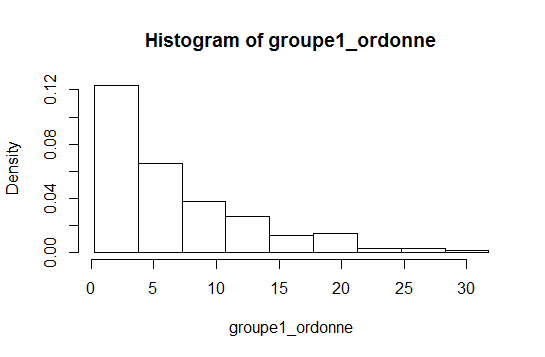
\includegraphics[width = 7cm]{{{graphics/q2_1-groupe1}.eps}}
\label{fig2}
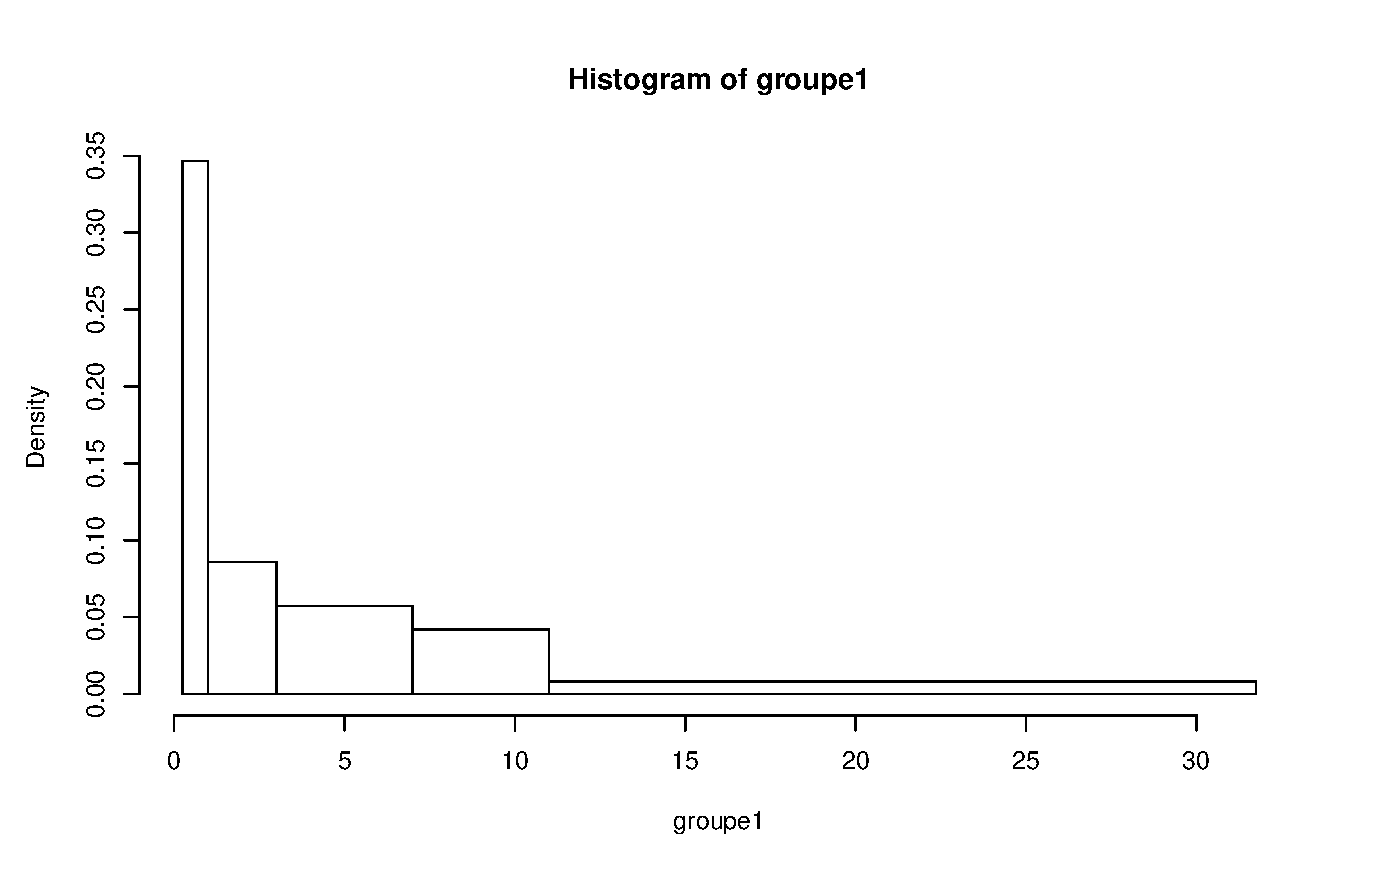
\includegraphics[width = 7cm]{{{graphics/q2_1-groupe1b}.eps}}
\label{fig2}
\end{center}



\begin{center}
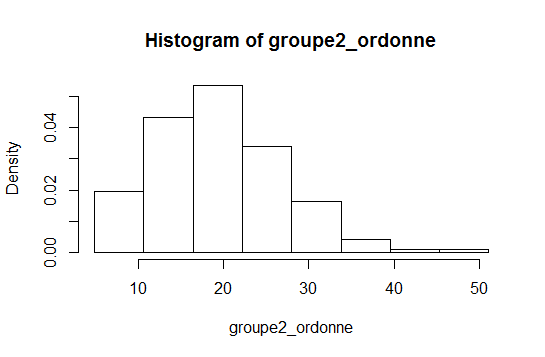
\includegraphics[width = 7cm]{{{graphics/q2_1-groupe2}.eps}}
\label{fig2}
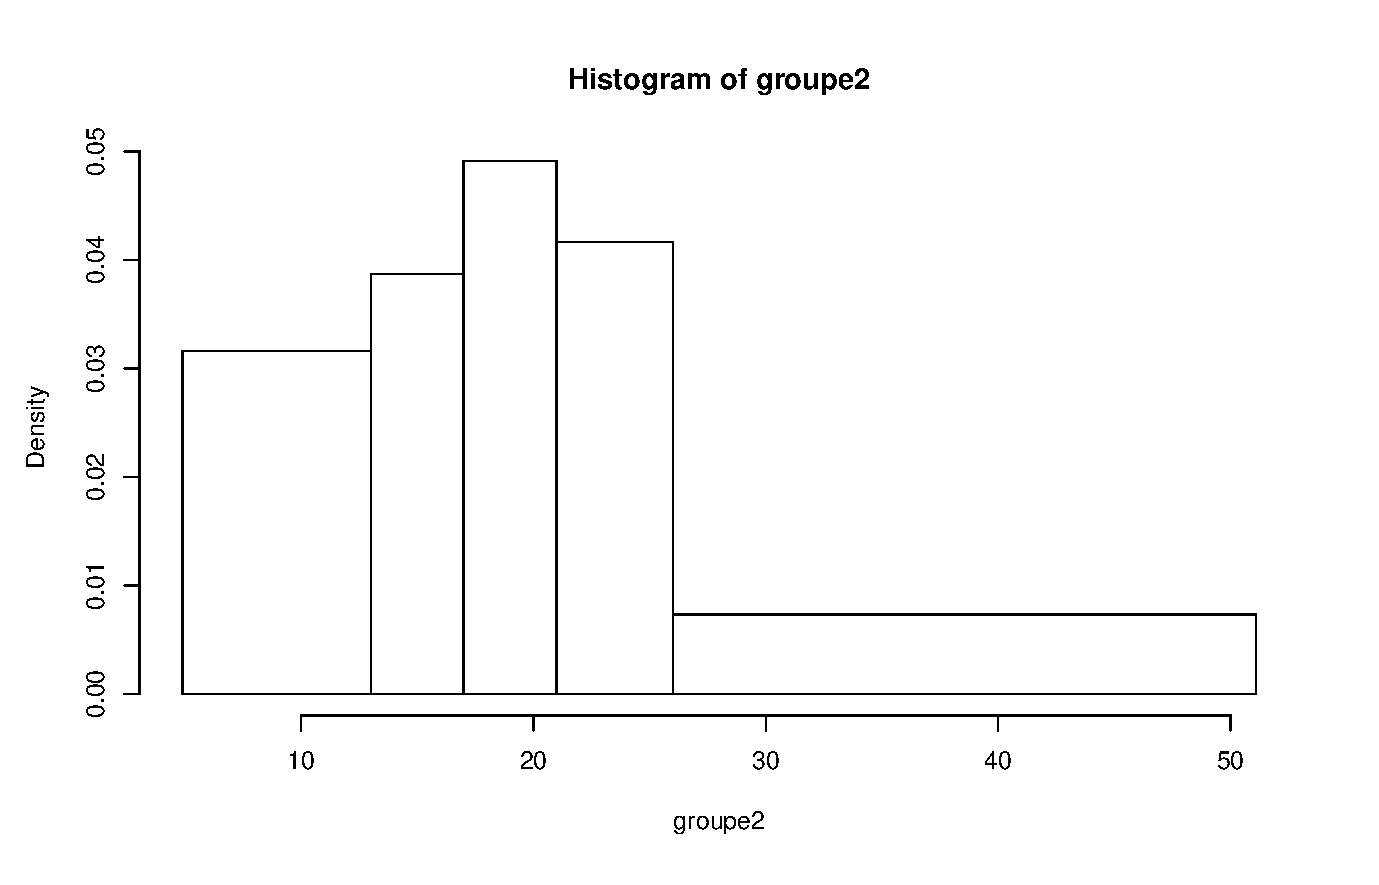
\includegraphics[width = 7cm]{{{graphics/q2_1-groupe2b}.eps}}
\label{fig2}
\end{center}


\item Les lois géométrique et binomiale négative sont-elles des modèles plausibles pour ces deux jeux de données ? Pour chaque jeu de données, choisir un modèle pertinent, estimer ses paramètres de toutes les façons possibles et, quand c'est possible, donner un intervalle de confiance asymptotique de seuil $\alpha=5\%$ pour ces paramètres.

\textbf{Estimation graphique\\}
Pour le groupe 1: La loi géométrique est un modèle pertinent. En effet nous avons utilisés la méthode graphique, en traçant le graphe de probabilité avec les données.
\begin{center}
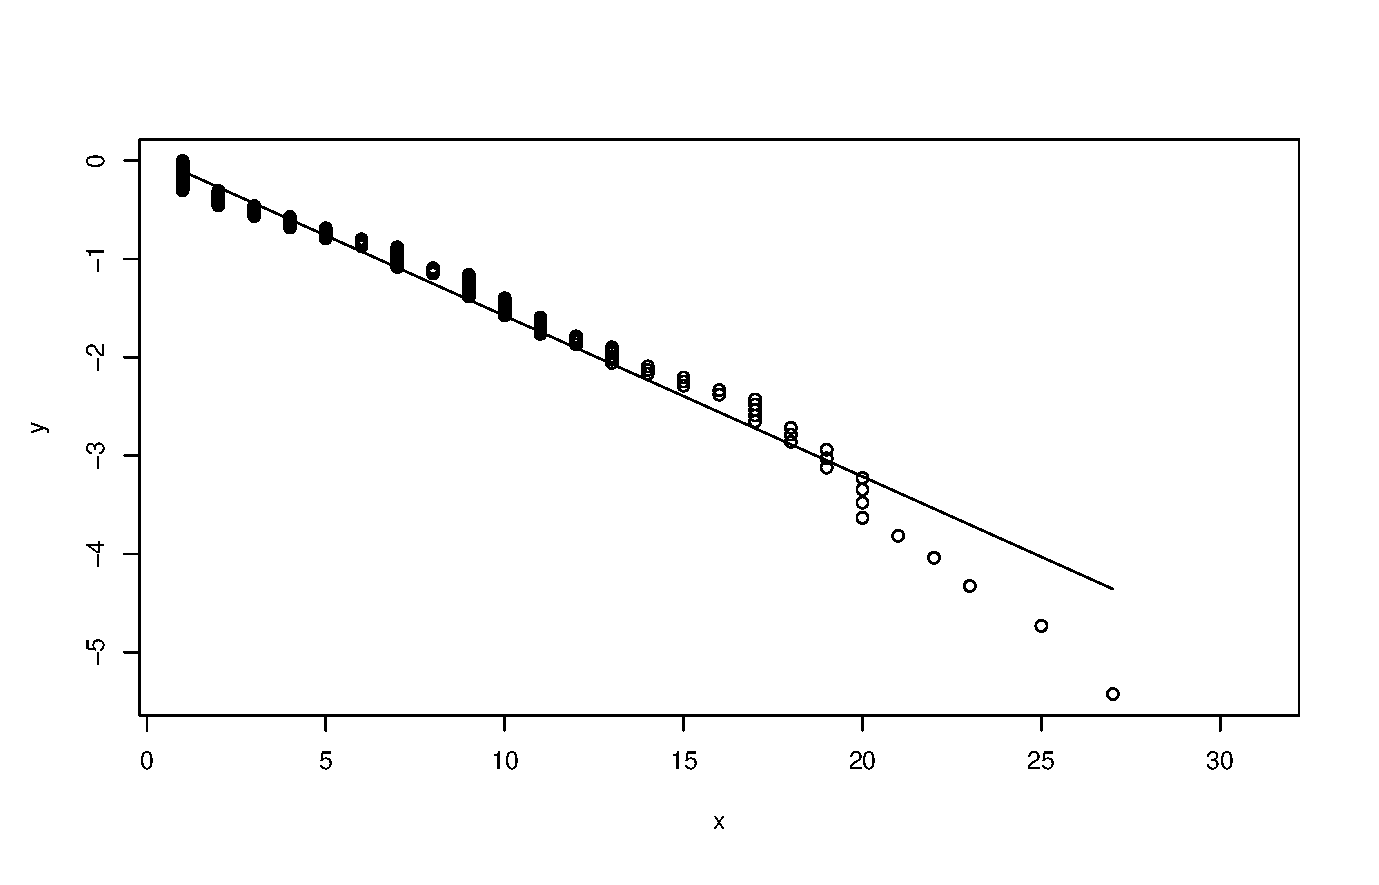
\includegraphics[width=15cm]{{{graphics/q2.2.1}.eps}}
\captionof{figure}{Graphe de probabilité pour la loi géométrique sur le groupe 1}
\label{fig1}
\end{center}
On constate que la droite est quasi-linéaire, ce qui montre que la loi géométrique est un modèle plausible. \\
D'après la question 1.3, on obtient une droite dont le coefficient directeur a est $a = ln(1-p) \Rightarrow p_{g_{1}} = 1 - e^{a} $ ce qui donne numériquement $ p=0,1507846 $\\
D'après la question 1.2, l'intervalle de confiance est: $ [0.1354829, 0.1723137]$. \\

\vspace{3mm}
Pour le groupe 2, nous utilisons la méthode de la question 1.4: \\
\begin{center}
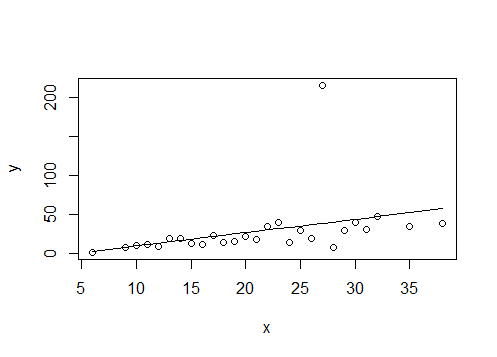
\includegraphics[width=15cm]{graphics/q2_2-groupe2.png}
\captionof{figure}{Graphe de probabilité pour la loi binomiale négative pour le groupe 2}
\label{fig3}
\end{center}
On constate que la loi binomiale négative est un modèle plausible pour le second groupe. \\
D'après la question $1.4(b)$, en traçant les points $\left( x, \dsp \frac{xP(x =X)}{P(X=x+1)} \right)$ on obtient une droite de pente $a = \dsp {1}{1-p} \Rightarrow p = 1 - \frac{1}{a}$ \\
Numériquement on obtient $ p_{g_{2}} = 0.4089586 $\\
Grâce à nos scripts R, on sait que le maximum de vraisemblance est atteint pour $r=5$

\textbf{\textit{Estimation avec la méthode des moments}}\\
En appliquant la méthode des moments au groupe 1 (question 1.1), on trouve $\tilde{p_n} = 0.1538983$ \\

\vspace{5mm}
En appliquant la méthode des moments au groupe 2 ( question 1.5), on trouve $\tilde{p_n} = 0.2476021 $  et $\tilde{r_n} = 4.887194$ or $\tilde{r_n}$ doit être un entier donc $\tilde{r_n} = 5$
D'après la question 2.2, $ IC = [0.2458528,0.260781]$


\item Pour les deux jeux de données, estimer le nombre moyen de fixations nécessaires pour identifier le type du texte lu et estimer la probabilité que ce nombre soit supérieur à 10. Quelle conclusion générale tirer de cette analyse ? \\
\textbf{Réponse :\\}
A la question précédente, nous avons calculé les différents paramètres nous permettant de déterminer l'espérance de chacune des lois et donc de déterminer le nombre moyen de fixations nécessaires pour identifier le type du texte lu. \\


Nous testons l'hypothèse $H_0$ "$m \geq 10$" contre $H_1$ "$m < 10$". \\
On utilise le théorème central-limite et le test de student:\\
$ W = \{n^{1/2} \frac{X_n - 10}{S'_n} > t_{n-1, 2\alpha}\}$
La p-valeur est: $1 - F_{St(n-1)}(n^{1/2} \frac{X_n - 10}{S'_n})$

Pour le groupe 1, la moyenne empirique est: $6.631977 $ \\
Pour le groupe 2, la moyenne empirique est $19.7381$ (méthode numérique) \\
La méthode graphique donnait $12.22618$, qui n'est pas une valeur pertinente. Nous ne retiendrons pas cette dernière, mais la première. \\

Nous calculons la p-valeur avec la formule et la t.test. \\
Pour le groupe 1, la p-valeur est: $2.2\times10^{-16}$ \\
Pour le groupe 2, la p-valeur est: $1$ \\

Conclusion: les p-valeurs nous montrent que nous devons rejeter l'hypotèse $H_1$ pour le groupe 1, et l'hypothèse $H_0$ pour le groupe 2.


% Intéressons nous à la probabilité que le nombre de fixations nécessaires pour déterminer le type de texte soit supérieur à 10, pour cela on compte le nombre de valeurs supérieures à 10 dans chacun des échantillons. \\
% Pour le groupe 1 : $P(x \geq 10) = 0.2511013 $ \\²
% Pour le groupe 2: $P(x \geq 10) = 0.9285714$\\
%
% Tout d'abord notons que l'échantillon pour le groupe 2 ne comporte que 168 valeurs, ce qui n'est pas assez pour faire de bonnes approximations graphiques ce qui explique la différence entre les valeurs obtenues par méthode graphique et méthode des moments. De plus certaines valeurs semblent abérrantes au vu du graphe de probabilités pour la loi binomiale négative. \\
% On remarque également que la majorité du  groupe deux est beaucoup plus rapide pour identifier le type du texte puisque la probabilité pour qu'il l'identifie en moins de 10 essais est supérieure à 0.90 contre un petit 0.25 pour le premier groupe.\\
% Mais le nombre de mots nécessaires pour identifier le type de texte varie beaucoup plus pour le groupe 2 puisque le nombre moyen de mots est 12 avec 90 pourcent du nombre de mots nécessaires inférieur à 10. Cela signifie que certaines personnes ont eu besoin de beaucoup de mots pour déterminer le type de texte.\\
% A l'inverse au sein du groupe 1, le nombre de mots nécessaires est plus centré autour de la valeur de 10, il y a très peu de personnes ayant eu besoin de beaucoup de mots.
\end{enumerate}
%%%%%%%%%%%%%%%%%%%%%%%%%%%%%%%%%%%%%%%%%%%%%%%%%%%%%%%%%%%%%%%
\section{Vérifications expérimentales à base de simulations}
%%%%%%%%%%%%%%%%%%%%%%%%%%%%%%%%%%%%%%%%%%%%%%%%%%%%%%%%%%%%%%%


\begin{enumerate}

\renewcommand{\labelenumi}{\arabic{section}.\arabic{enumi}.}

\item Choisir $p$, $n$, $m$ et $\alpha$. Simuler $m$ d'échantillons de taille $n$ de la loi ${\cal G}(p)$. Pour chacun d'entre eux, calculer l'intervalle de confiance asymptotique de seuil $\alpha$ pour $p$ obtenu dans la question 2.2. Comparer la proportion d'intervalle contenant la vraie valeur de $p$ à $1-\alpha$. Quel est l'impact du choix des valeurs de $p$, $n$, $m$ et $\alpha$ ?

Paramètre fixés pour cette simulation, $p=0.15$, $m=1000$, $\alpha = 0.05$\\

\begin{center}
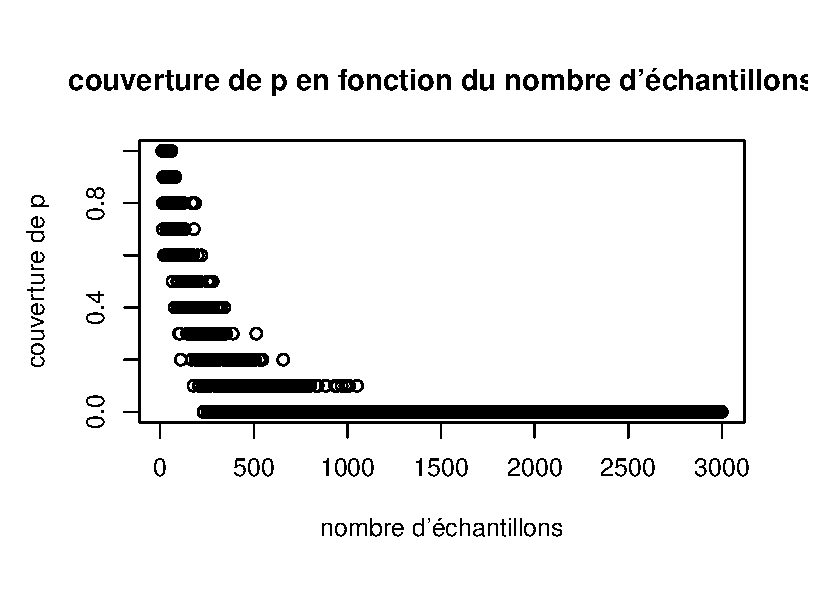
\includegraphics[width=15cm]{{{graphics/q3.1-graphe1}.eps}}
\end{center}

On remarque que plus n est grand, plus la probabilité que  p appartienne à l'intervalle de confiance est proche de la valeur théorique, à savoir de $1-\alpha$, donc plus l'estimation est précise.

\vspace{5mm}
Paramètres fixés pour cette simulation, $n=1000$, $m=1000$, $\alpha =0.05$ \\
\begin{center}
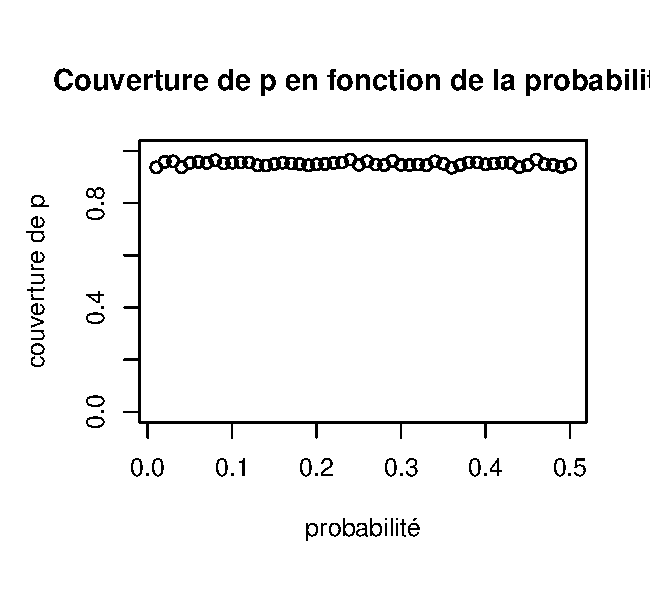
\includegraphics[width=15cm]{{{graphics/q3.1-graphe_2}.eps}}
\end{center}
Grâce à ce graphe on remarque que la probabilité de l'échantillon n'influe pas sur la probabilité de se tromper en affirmant que p appartient à l'intervalle de confiance.

\vspace{5mm}


Paramètres fixés pour cette simulation, $n=1000$, $p=0.15$, $\alpha = 0.05$ \\
\begin{center}
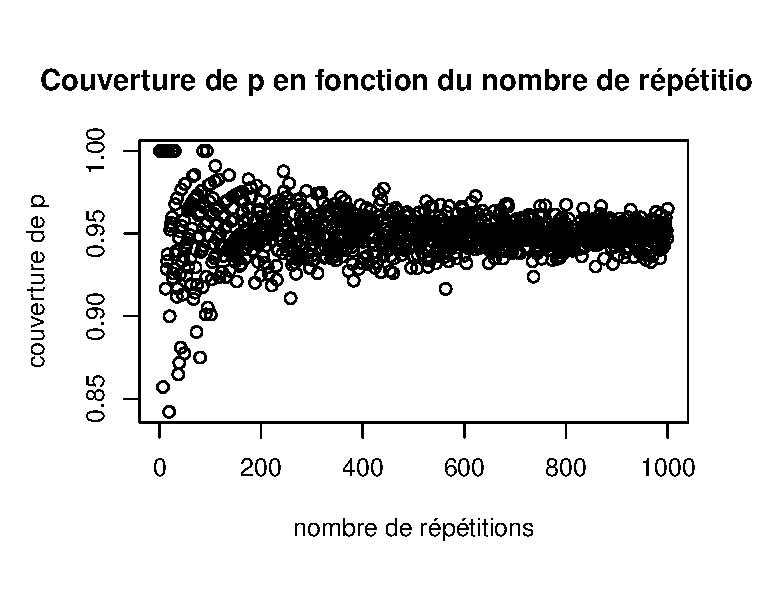
\includegraphics[width=15cm]{{{graphics/q3.1-graphe3}.eps}}
\end{center}

\vspace{5mm}


Paramètres fixés pour cette simulation, $n=10000$, $p=0.15$, $p=0.15$ \\

\begin{center}
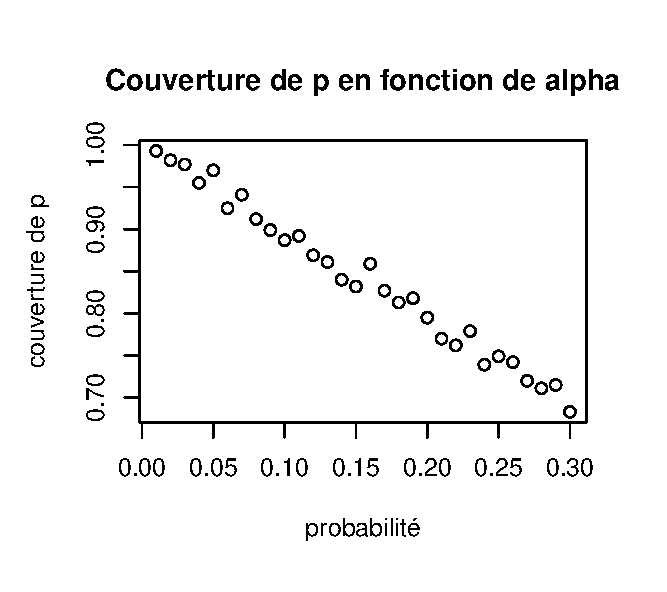
\includegraphics[width=15cm]{{{graphics/q3.1-graphe4}.eps}}
\end{center}

Grâce au graphique, on voit que la probabilité que p appartienne à l'intervalle de confiance vaut $1-\alpha$. En augmentant alpha, on diminue le nombre de p dans l'intervalle de confiance.

\vspace{3mm}

\item Vérification de la loi faible des grands nombres. Simuler $m$ échantillons de taille $n$ de la loi ${\cal G}(p)$. Calculer le nombre de fois où l'écart en valeur absolue entre la moyenne empirique et l'espérance de la loi simulée est supérieure à un $\epsilon$ à choisir. Faire varier $n$ et conclure.

\begin{center}
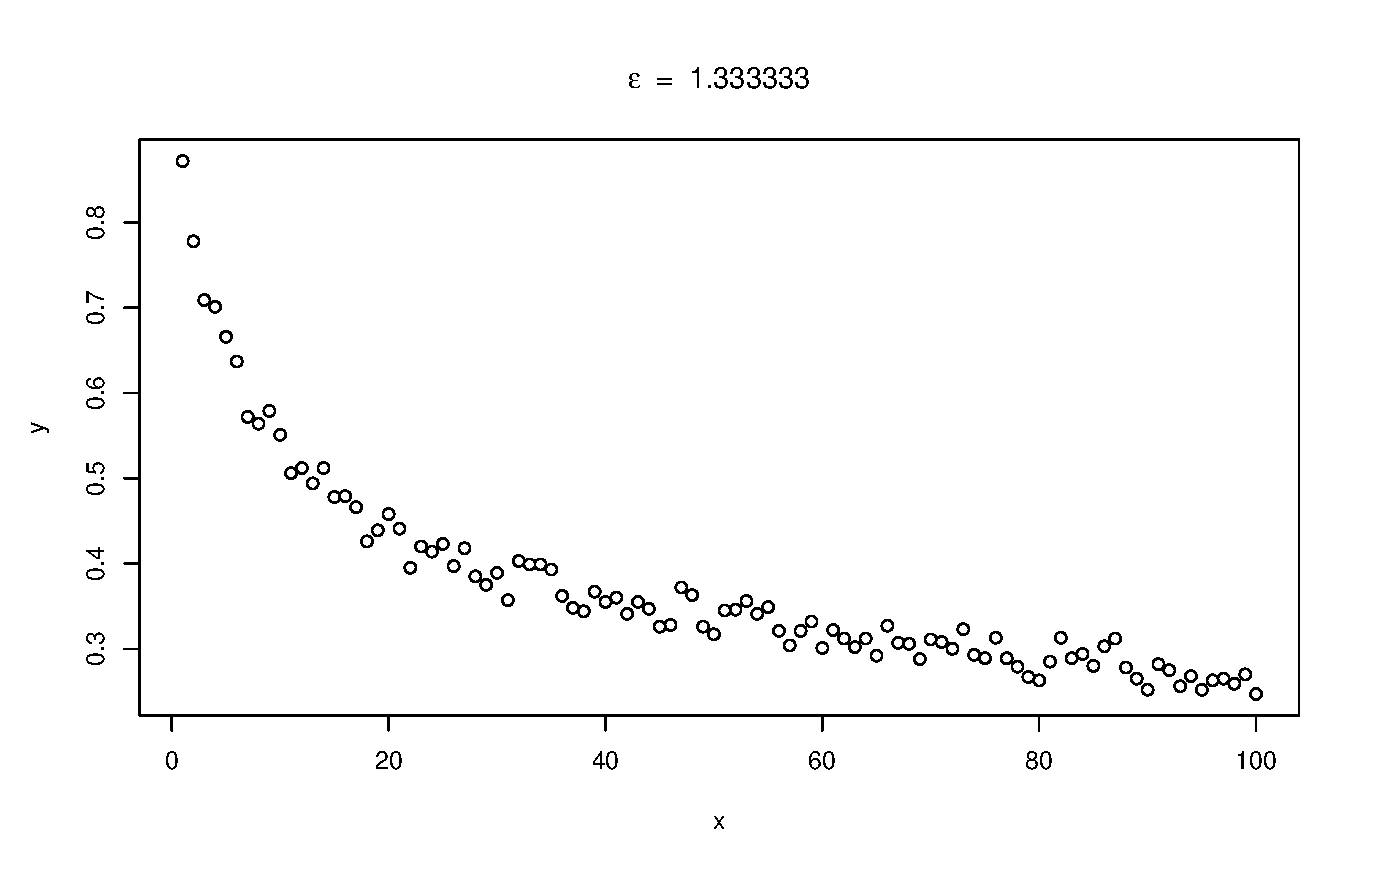
\includegraphics[width=7cm]{{{graphics/q3.2.d}.eps}}
% \captionof{figure}{Graphe de probabilités avec la méthode basée sur la fonction de répartition}
\label{fig5}
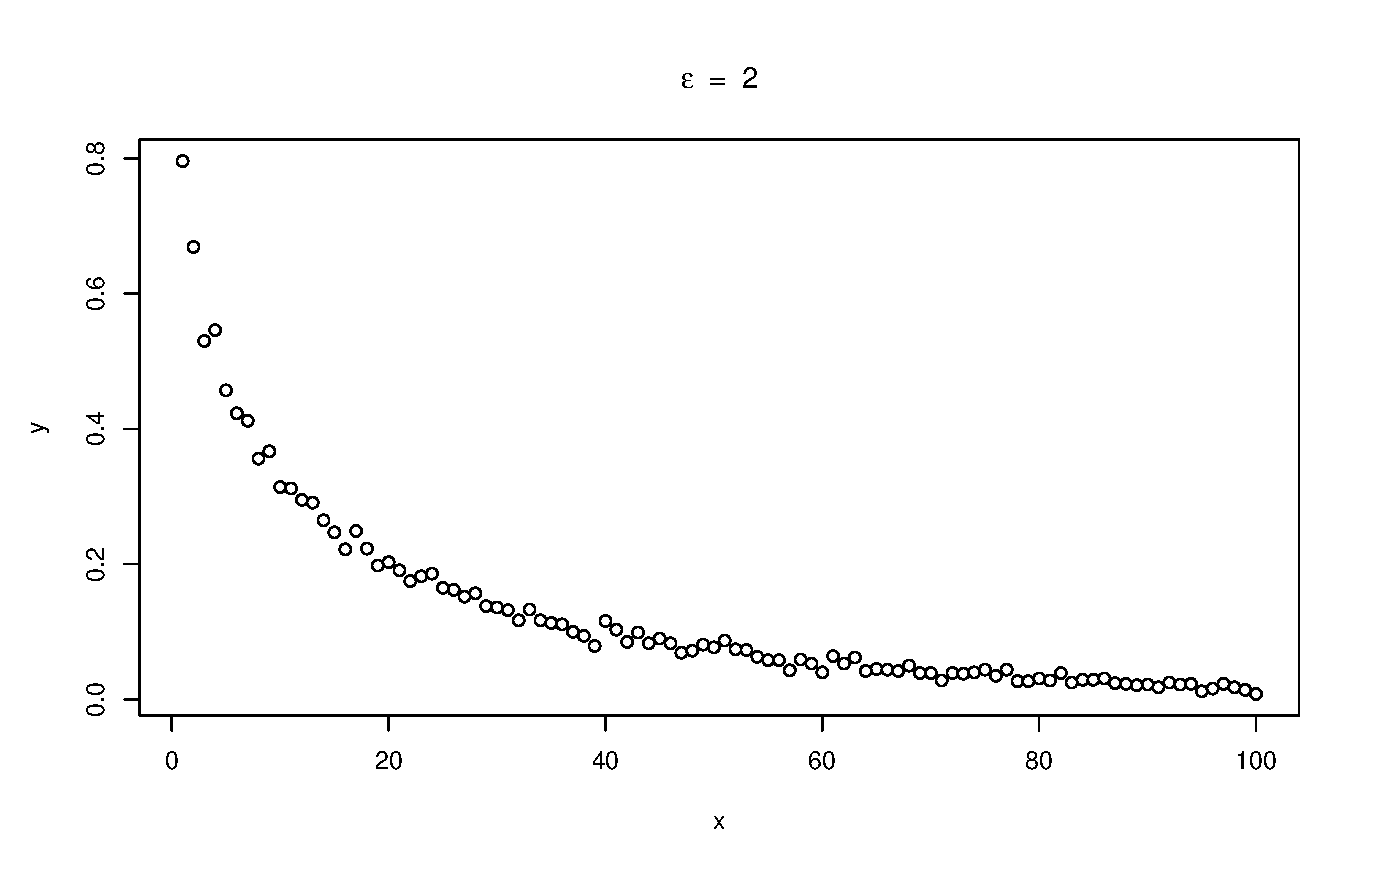
\includegraphics[width=7cm]{{{graphics/q3.2.a}.eps}}
% \captionof{figure}{Graphe de probabilités avec la méthode basée sur la fonction de répartition}
\label{fig6}
\end{center}

\begin{center}
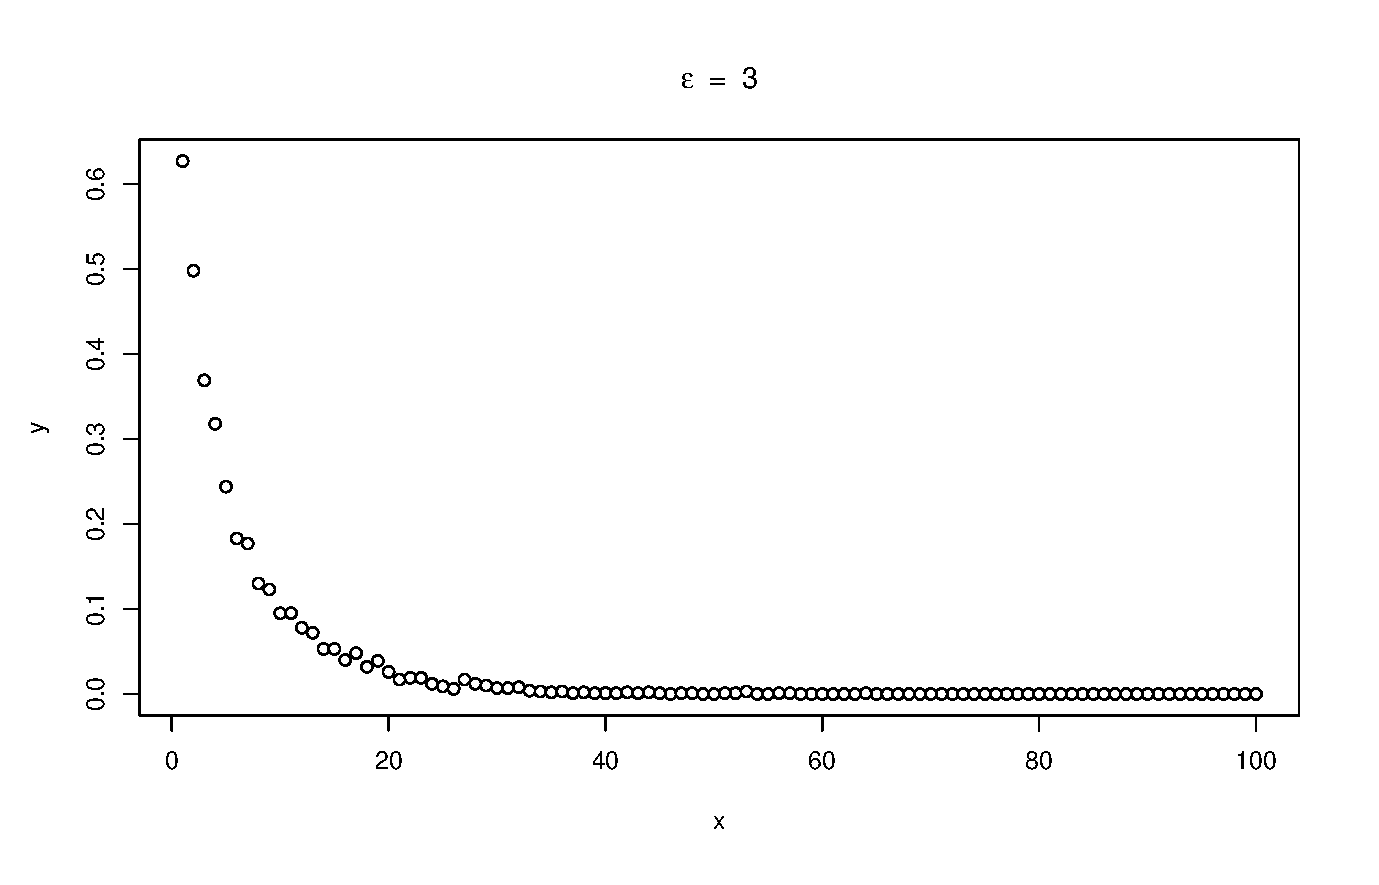
\includegraphics[width=7cm]{{{graphics/q3.2.b}.eps}}
% \captionof{figure}{Graphe de probabilités avec la méthode basée sur la fonction de répartition}
\label{fig7}
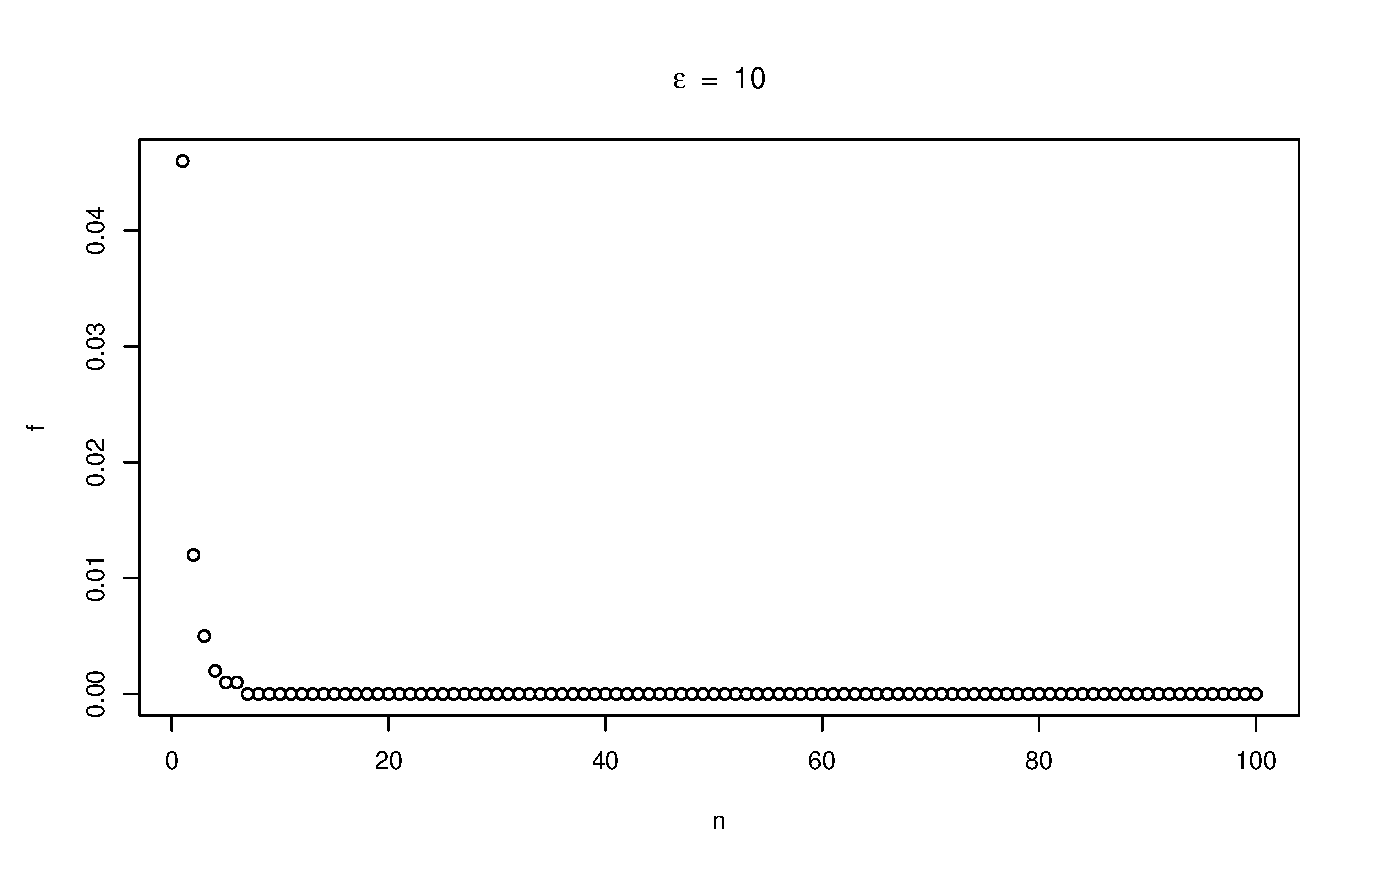
\includegraphics[width=7cm]{{{graphics/q3.2.c}.eps}}
% \captionof{figure}{Graphe de probabilités avec la méthode basée sur la fonction de répartition}
\label{fig8}
\end{center}

Quelque soit $\epsilon$ strictement positif, nous constatons empiriquement avec la loi ${\cal G}(p)$ que quand n (en abscisses) devient suffisemment grand, la fréquence de dépassement de la valeur absolue de l'écart entre la moyenne empirique devient négligeable.
La loi faible des grands nombres.

\vspace{3mm}

\item Vérification du théorème central-limite. Simuler $m$ échantillons de taille $n$ de la loi ${\cal G}(p)$. Sur l'échantillon des $m$ moyennes empiriques, tracer un histogramme et un graphe de probabilités pour la loi normale. Faire varier $n$ en partant de $n=5$ et conclure.

\vspace{3mm}

\begin{center}
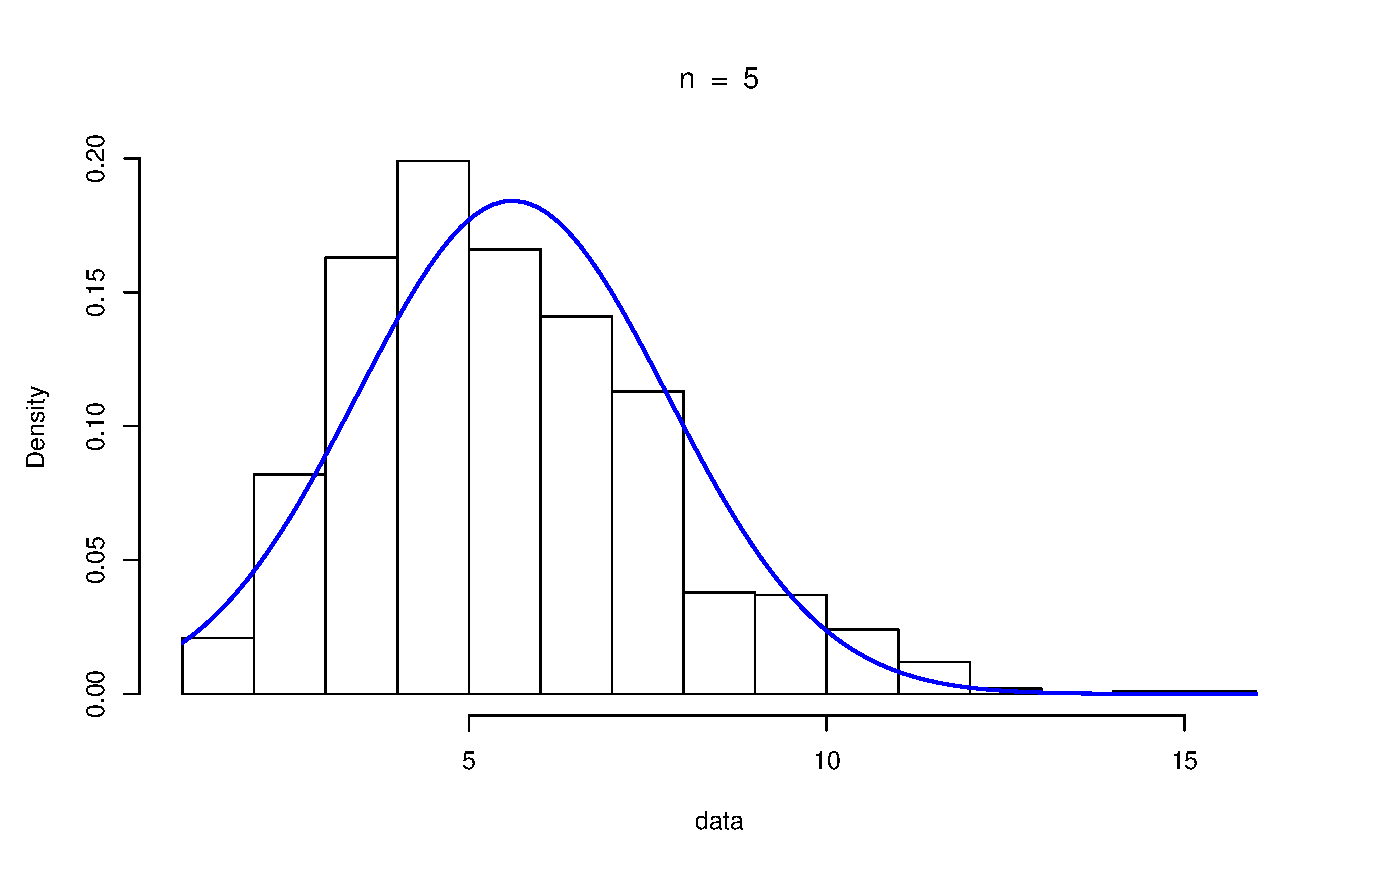
\includegraphics[width=7cm]{{{graphics/q3.3a}.eps}}
% \captionof{figure}{Graphe de probabilités avec la méthode basée sur la fonction de répartition}
\label{fig5}
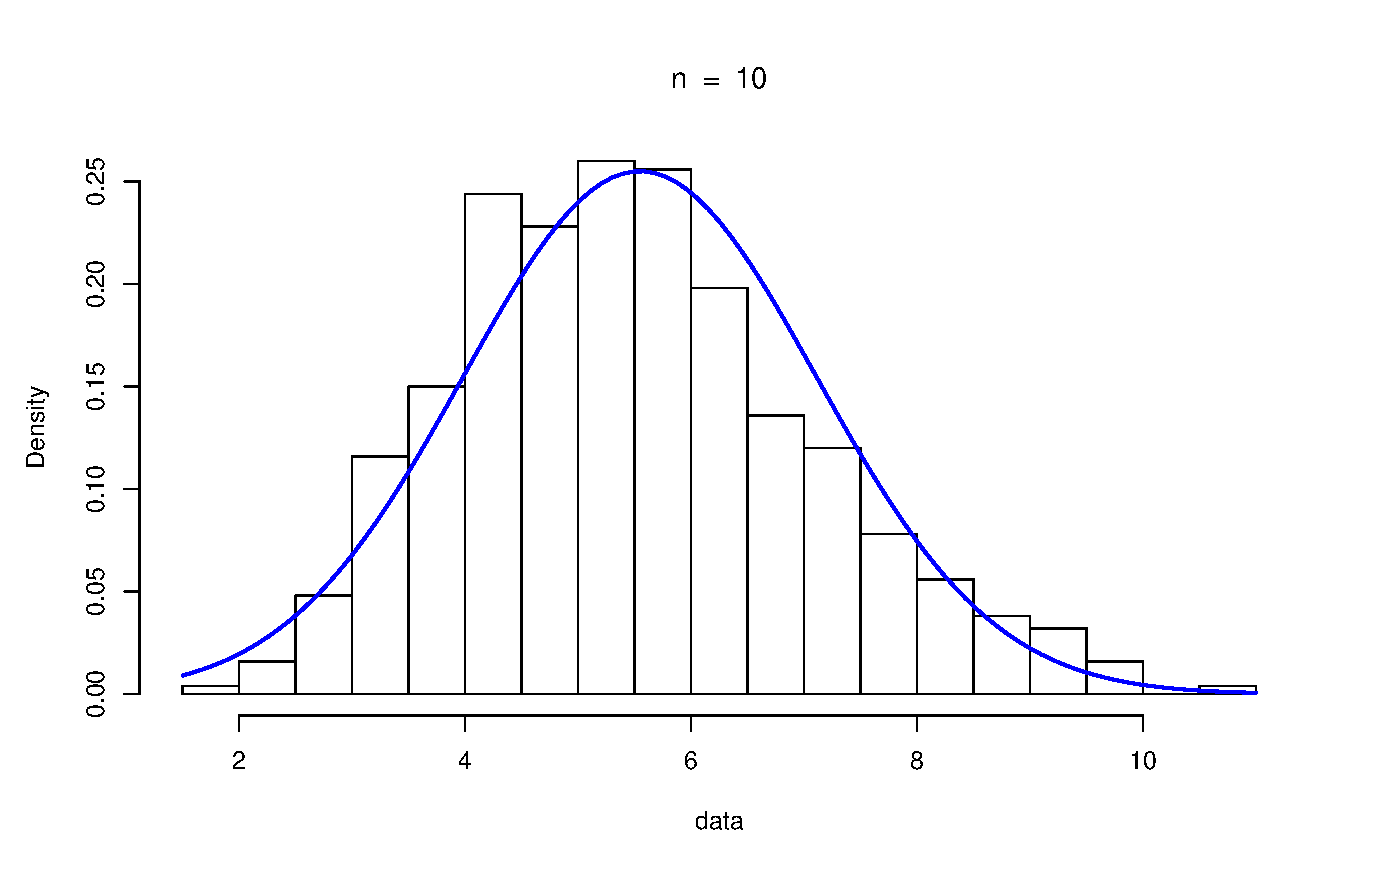
\includegraphics[width=7cm]{{{graphics/q3.3b}.eps}}
% \captionof{figure}{Graphe de probabilités avec la méthode basée sur la fonction de répartition}
\label{fig6}
\end{center}

\begin{center}
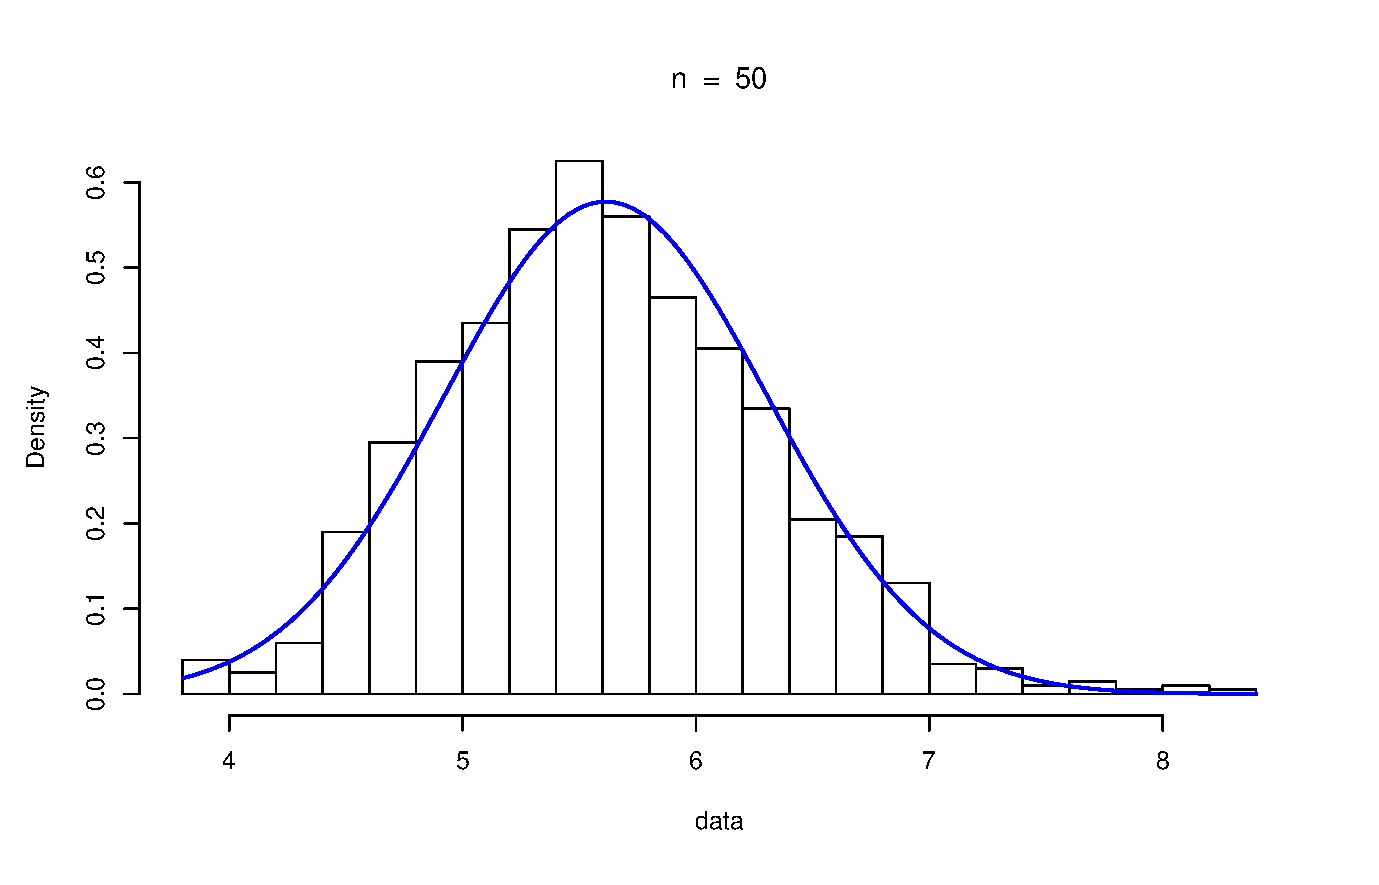
\includegraphics[width=7cm]{{{graphics/q3.3c}.eps}}
% \captionof{figure}{Graphe de probabilités avec la méthode basée sur la fonction de répartition}
\label{fig5}
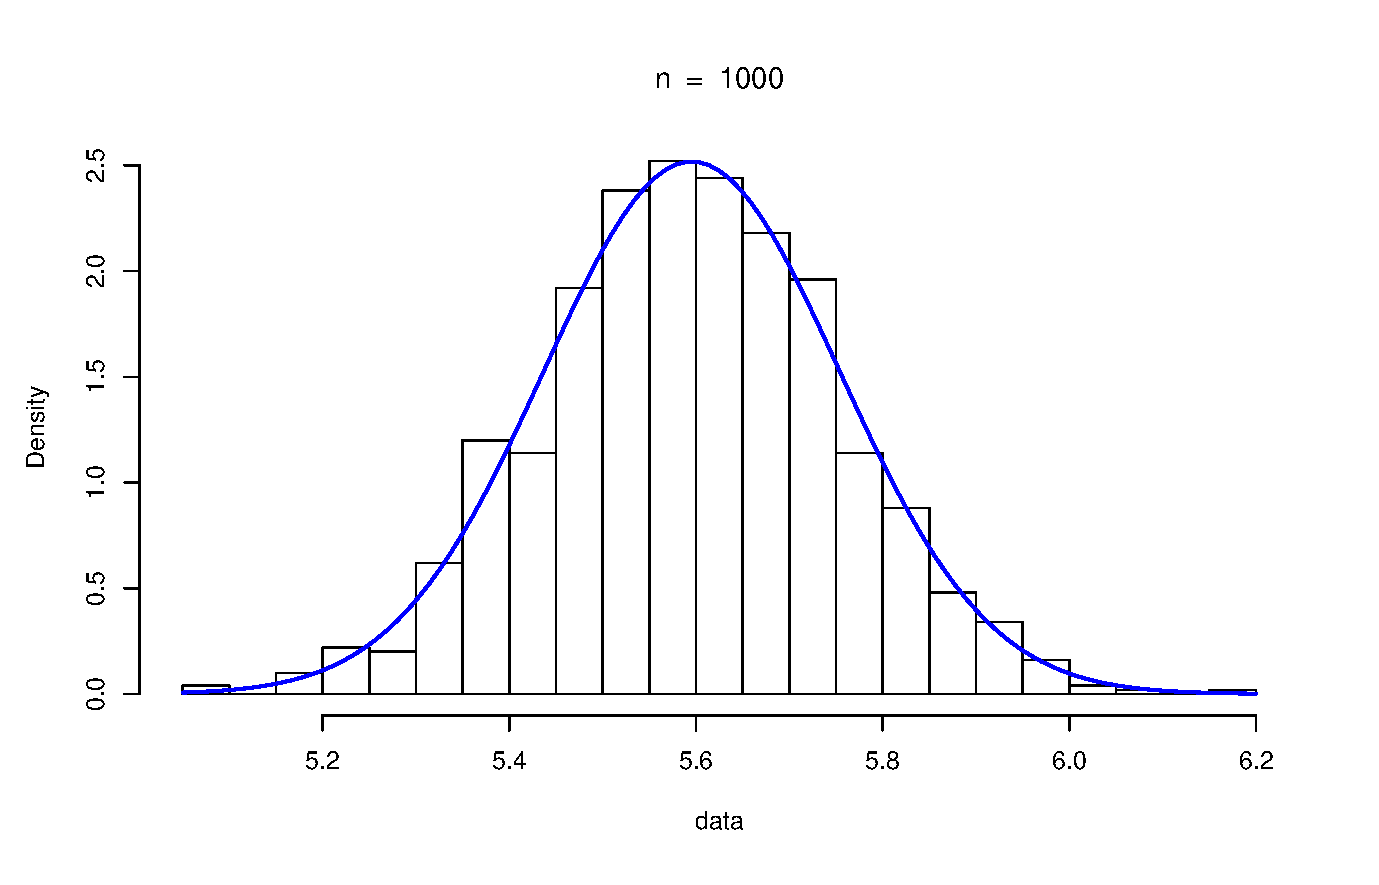
\includegraphics[width=7cm]{{{graphics/q3.3d}.eps}}
% \captionof{figure}{Graphe de probabilités avec la méthode basée sur la fonction de répartition}
\label{fig5}
\end{center}

On constate que l'histogramme tend vers le graphe de probabilité de la loi normale lorsque n devient grand. \\
La convergence est très rapide, $n=100$ s'approche très bien de la loi normale.

\vspace{3mm}

\item Choisir $r$, $p$, $n$ et $m$. Simuler $m$ échantillons de taille $n$ de la loi ${\cal BN}(r,p)$. Pour chaque échantillon, calculer les estimateurs des moments de $r$ et $p$, $\tilde{r}_n$ et $\tilde{p}_n$. Utilisez ces simulations pour évaluer le biais et l'erreur quadratique moyenne de ces estimateurs. Faire varier $n$ et commenter les résultats.

\vspace{5mm}
Nous avons évalué le biais et l'erreur quadratique de $\tilde{p_n}$ et $\tilde{r_n}$ avec les paramètres suivants : $p = 0.2$, $m=1000$, $r=5$

\begin{center}
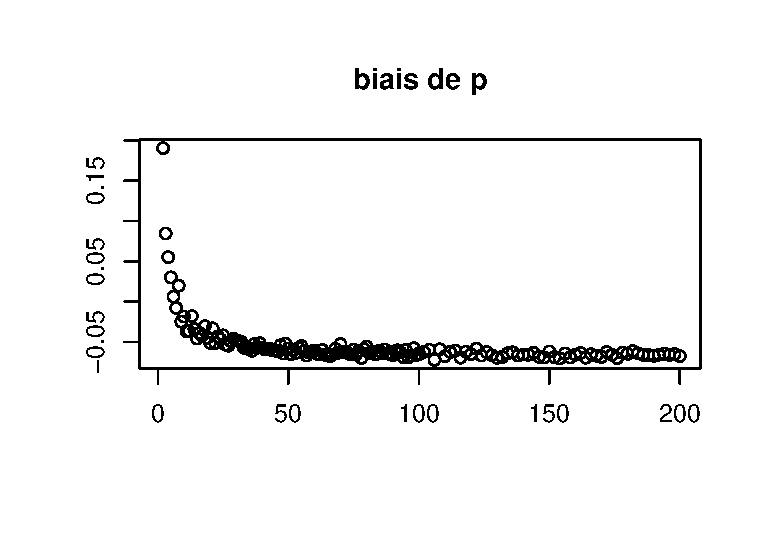
\includegraphics[width=7cm]{{{graphics/q3.4-graphe1}.eps}}
% \captionof{figure}{Graphe de probabilités avec la méthode basée sur la fonction de répartition}
% \label{fig5}
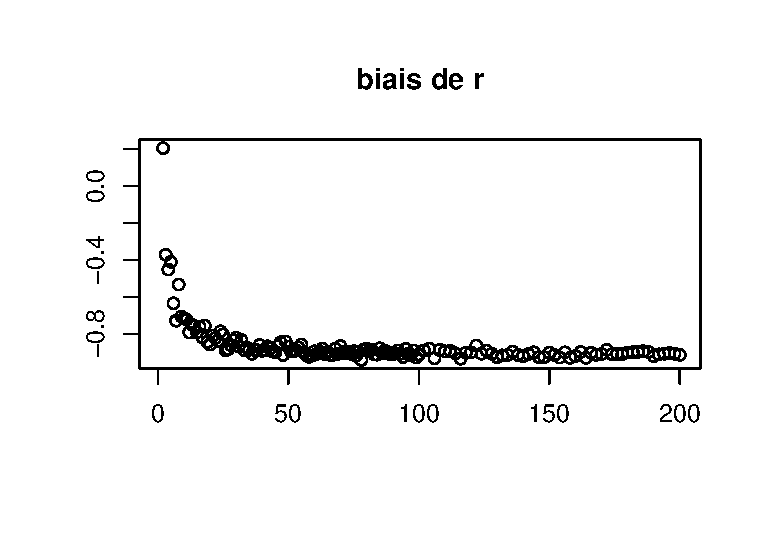
\includegraphics[width=7cm]{{{graphics/q3.4-graphe2}.eps}}
% \captionof{figure}{Graphe de probabilités avec la méthode basée sur la fonction de répartition}
% \label{fig6}
\end{center}

\begin{center}
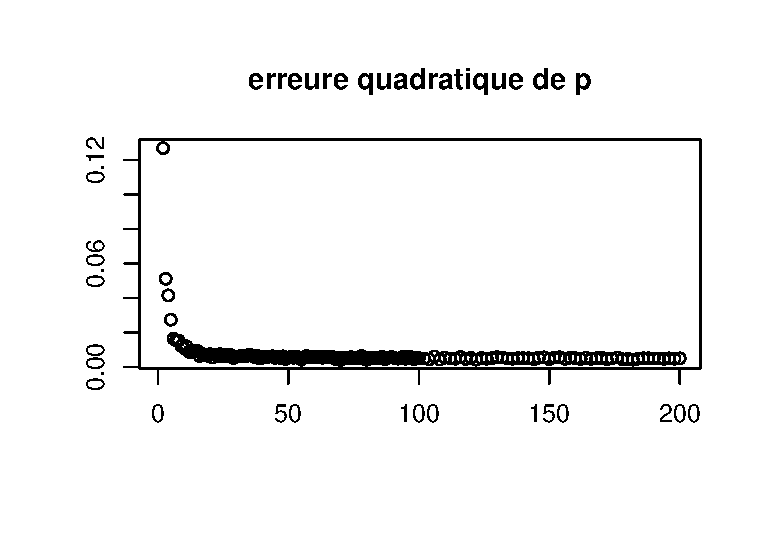
\includegraphics[width=7cm]{{{graphics/q3.4-graphe3}.eps}}
% \captionof{figure}{Graphe de probabilités avec la méthode basée sur la fonction de répartition}
% \label{fig5}
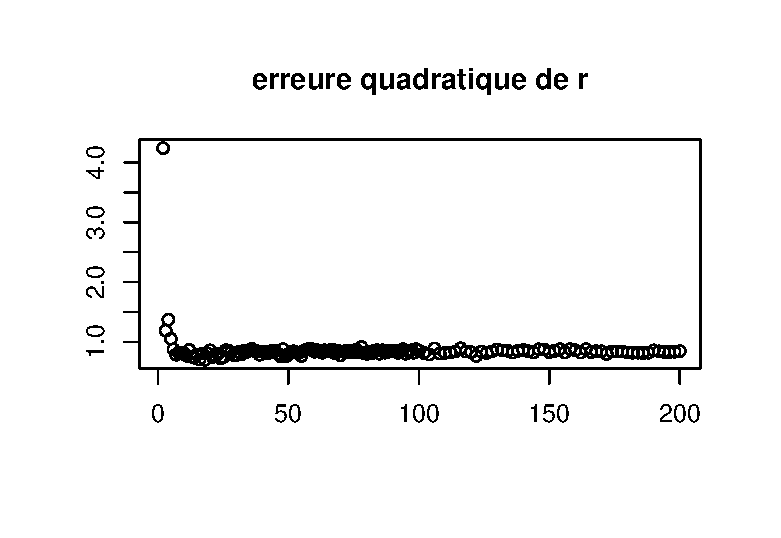
\includegraphics[width=7cm]{{{graphics/q3.4-graphe4}.eps}}
% \captionof{figure}{Graphe de probabilités avec la méthode basée sur la fonction de répartition}
% \label{fig5}
\end{center}

On constate que les estimateurs de p et de r sont biaisés. Il ne sont même pas asymptotiquement sans biais. \\
Cependant les erreurs quadratiques des estimateurs sont nulles.
Ainsi on pourrait imaginer tenter les corriger (du moins asymptotiquement), en effectuant des calculs dans la mesure du possible. \\
Nous n'avons pas réussi à faire cette étape malheureusement. \\
\end{enumerate}

\end{document}
